%documentclass sets the look of the whole document. you can try changing it around with the two commented out examples.

\documentclass{article}
\usepackage{graphicx}

%\documentclass{proc}
%\documentclass{beamer}


\title{Here is an example of how to use sub-files in LaTeX}

\author{NOP}

\begin{document}
\maketitle

%to include the table of contents just uncoment the line below. The newpage line would move the start of the document on the next page after the table of contents.
%\tableofcontents
%\newpage

\section{Shared Part}

This could be the Shared Part of the document. It is designed to be written by all members of the team.

Each member should ideally write their details in the table of contributors in the Shared Part of the document.

\subsection{Comments from the first student}
Well, the module has happened, isn't that great, we have the ability to remember a whole bunch of \textbf{bunches} of diagram types, \textbf{bought} a book for the expected reading to find out that all of the expected reading was provided with the sources of these documents looking \textbf{less legitimate} each passing week. But the labs, for the \textbf{labs} and the teamwork it has all been worth it.


\subsection{Comments from the second student}
This is the first subsection. Do not forget to include the best parts about the module as well as what you did not like about Max Wilson during the term.

\subsection{Comments from the third student}
This is the first subsection. Do not forget to include the best parts about the module as well as what you did not like about Max Wilson during the term.

\subsection{Comments from the forth student}
This is the first subsection. Do not forget to include the best parts about the module as well as what you did not like about Max Wilson during the term.

\subsection{Comments from the fifth student}
This is the first subsection. Do not forget to include the best parts about the module as well as what you did not like about Max Wilson during the term.

\subsection{Table of Contributors}


If you want to move a table around you will need to put some parameters in square brackets, if you want it exactly where it is positioned in the text editor just uncomment the [h] below, just after begin{table}

This is the table of contributors (Table~\ref{authors}):
\begin{table}[h]
\centering
\caption{People in the Group}
\label{authors}
\begin{tabular}{|l|l|}
\hline
\textbf{Name} & \textbf{ID} \\
\hline Joshua 
& 4297979\\ 
\hline
& \\
\hline
& \\
\hline
& \\
\hline
& \\
\hline
\end{tabular}
\end{table}
\newpage

\section{First Member}
This is the section dedicated to one of the team members, and it should be written individually . It can include a range of things; first subsection is a space for you to point out the strengths and weaknesses of the module, including complaints about the module coordinator Max Wilson. The second section should have a selfie image with Max! The last part of it is the most important one. You will need to write a paragraph about what you have learned in this module. You can write it in \textbf{Bold} if you want or you can use other fonts. 

Please do not forget:
\begin{itemize}
	\item First paragraph should have your comments about the module
	\item Second one, a selfie img with Max
	\item Last one, what you learned in this module.
\end{itemize}

\subsection{Comments about the module}

Well, the module has happened, isn't that great, we have the ability to remember a whole bunch of \textbf{bunches} of diagram types, \textbf{bought} a book for the expected reading to find out that all of the expected reading was provided with the sources of these documents looking \textbf{less legitimate} each passing week. But the labs, for the \textbf{labs} and the teamwork it has all been worth it.

The best part of the module has been the \textbf{labs} I have actually \textbf{enjoyed} working with my {fabulous} team. 

\subsection{Selfie with Max}

To include an image, you will need to remove the comments from the code below, place an image in the main folder, and do not forget to put the name of the image instead of ImgName. 


\begin{figure}[h]
\caption{Selfie with Max, inspired by Julian}
\centering

\includegraphics[width=1.0\textwidth]{maxSelfieJoshua.jpg}
\label{fig:selfie}
\end{figure}

You can then use the label of the figure to reference it later with the command ${\backslash}ref$. you can comment out the next line to see an example of how it works.

My selfie with Max is in  Figure~\ref{fig:selfie}.

\subsection{What I have learned in this module}

Teamwork makes the \textbf{dream} work. It is completely vital to plan to save development costs. You really need to talk to your clients, find out the requirements, make a specification, do low and high level planning. Create prototypes, liaise with the clients all of the way. then when you are sure that all of the specification is done, you plan the tests. Then you can finally start coding. All that is left is to do testing, first internally, then acceptance and user testing. Done!
\newpage
\section{Second Member}
This is the section dedicated to one of the team members, and it should be written individually . It can include a range of things; first subsection is a space for you to point out the strengths and weaknesses of the module, including complaints about the module coordinator Max Wilson. The second section should have a selfie image with Max! The last part of it is the most important one. You will need to write a paragraph about what you have learned in this module. You can write it in \textbf{Bold} if you want or you can use other fonts. 

Please do not forget:
\begin{itemize}
	\item First paragraph should have your comments about the module
	\item Second one, a selfie img with Max
	\item Last one, what you learned in this module.
\end{itemize}

\subsection{Comments about the module}
This is the first subsection. Do not forget to include the best parts about the module as well as what you did not like about Max Wilson during the term.
The FSE module has been very enjoyable. Despite me hearing that other students think it is the most boring module in terms of content, I do find some of it quite interesting, and the presentations from Max are well made and thought out. However, one thing I am not a fan of is the large number of expected reading set for the module. It's difficult to know what will important in the exam when given 5 pages of dense text in a pdf to read after every lecture.

\subsection{Selfie with Max}
Below is a selfie of me and Max Wilson
\begin{figure}[h]
\caption{Selfie with Max}
\centering
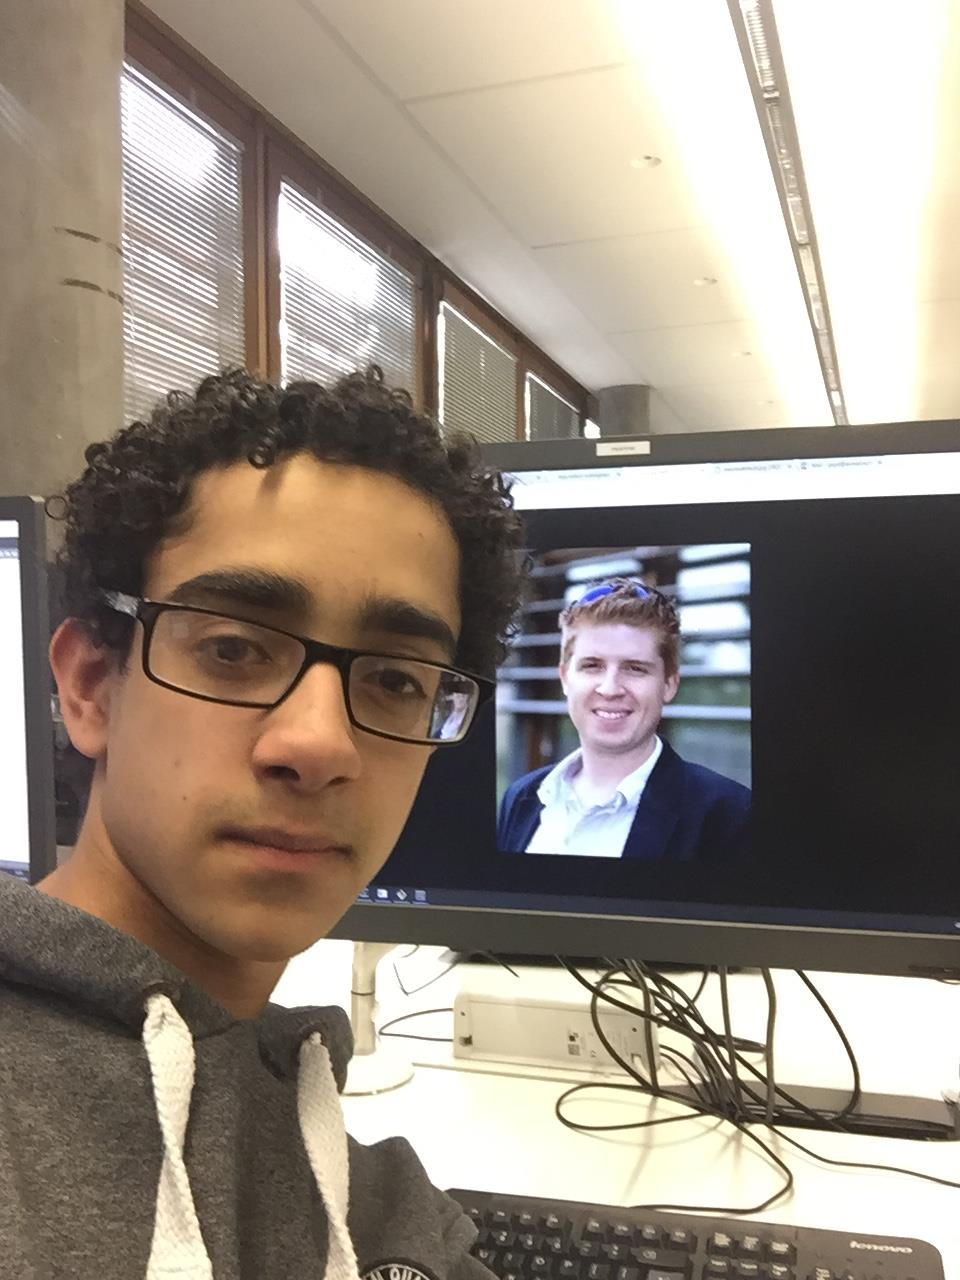
\includegraphics[width=0.5\textwidth]{psyit_real_selfie}
\label{fig:selfie}
\end{figure}

You can then use the label of the figure to reference it later with the command ${\backslash}ref.$ you can comment out the next line to see an example of how it works.

% My selfie with Max is in  Figure~\ref{fig:selfie}.

\subsection{What I have learned in this module}
In this module I have learnt about the various stages in the software engineering process as well as the different methodologies and strategies involved in creating successful software as a team.

Although we haven't done any real coding as teams as of yet, I have learnt a lot about how to work as team through the weekly lab sessions.


\newpage
\section{Third Member}
This is the section dedicated to one of the team members, and it should be written individually . It can include a range of things; first subsection is a space for you to point out the strengths and weaknesses of the module, including complaints about the module coordinator Max Wilson. The second section should have a selfie image with Max! The last part of it is the most important one. You will need to write a paragraph about what you have learned in this module. You can write it in \textbf{Bold} if you want or you can use other fonts. 

Please do not forget:
\begin{itemize}
	\item First paragraph should have your comments about the module
	\item Second one, a selfie img with Max
	\item Last one, what you learned in this module.
\end{itemize}

\subsection{Comments about the module}
This is the first subsection. Do not forget to include the best parts about the module as well as what you did not like about Max Wilson during the term.

Overall, this module has been fairly interesting. 

\subsection{Selfie with Max}

To include an image, you will need to remove the comments from the code below, place an image in the main folder, and do not forget to put the name of the image instead of ImgName. 

\begin{figure}[h]
\caption{Selfie with Max}
\centering
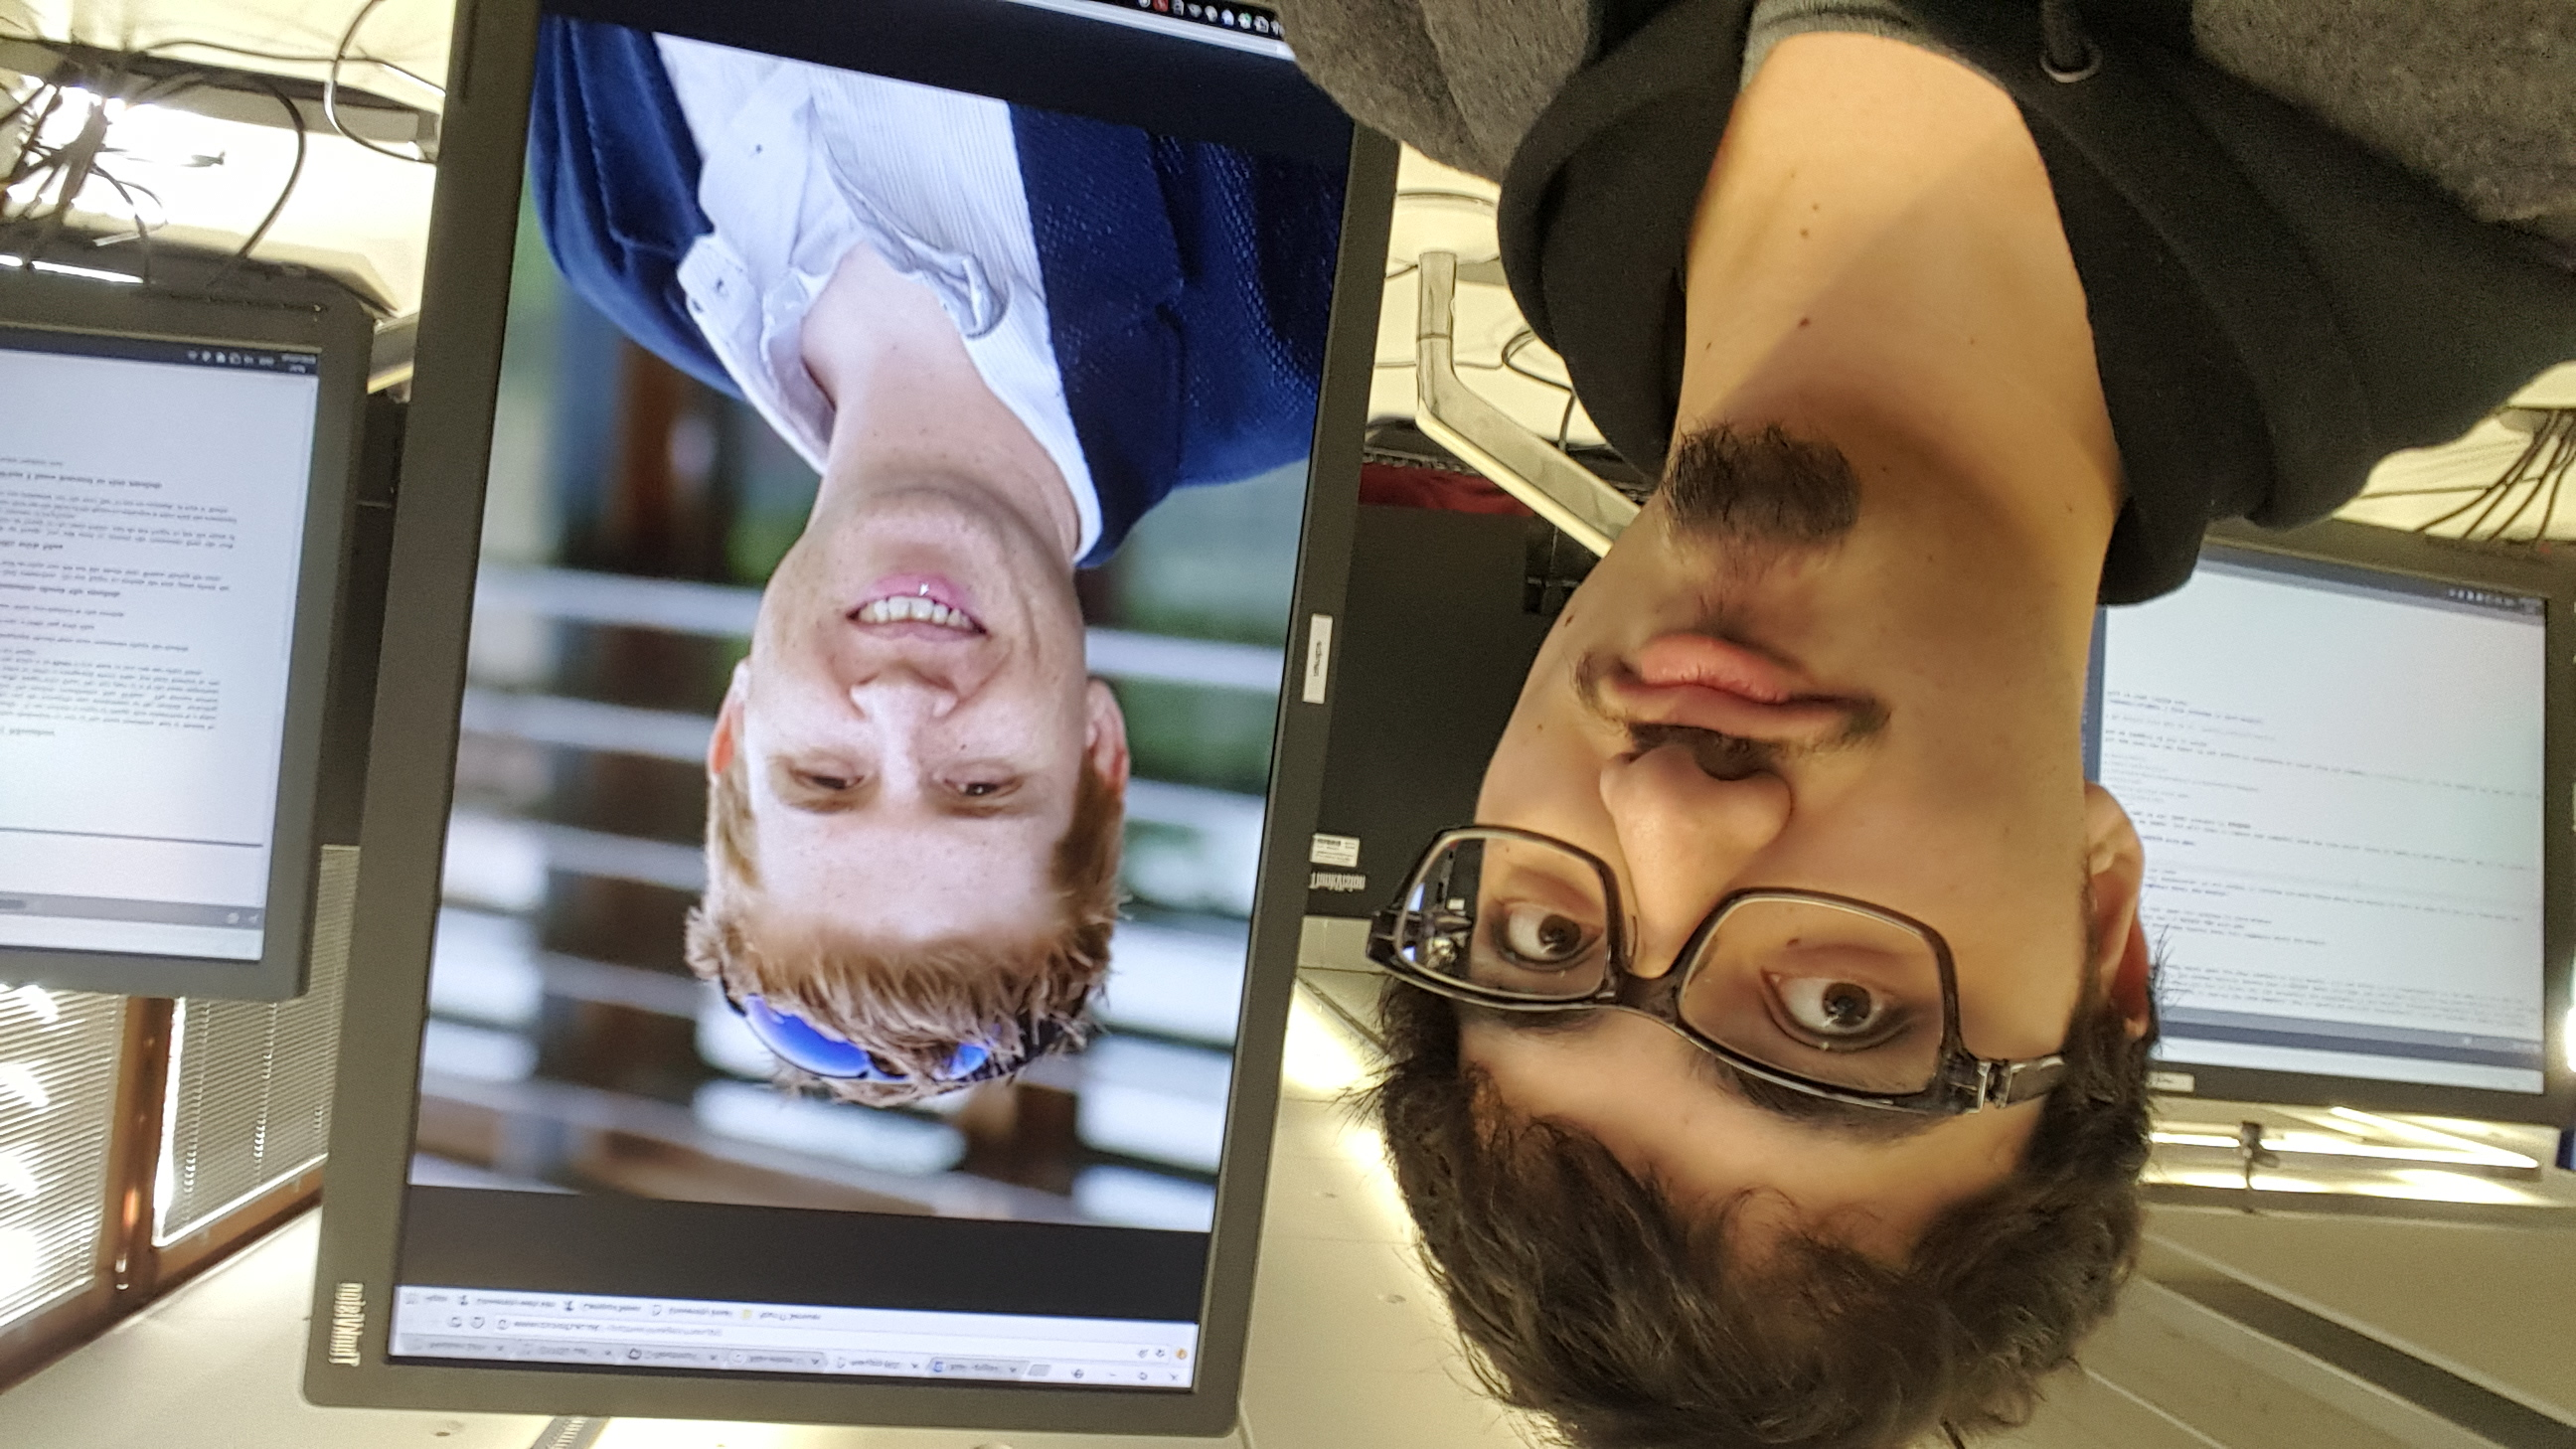
\includegraphics{psyjk4selfie}
\label{fig:selfie}
\end{figure}

%You can then use the label of the figure to reference it later with the command ${\backslash}ref$. you can comment out the next line %to see an example of how it works.

% My selfie with Max is in  Figure~\ref{fig:selfie}.

\subsection{What I have learned in this module}
This is some random text.


\newpage
\section{Fourth Member}
This is the section dedicated to one of the team members, and it should be written individually . It can include a range of things; first subsection is a space for you to point out the strengths and weaknesses of the module, including complaints about the module coordinator Max Wilson. The second section should have a selfie image with Max! The last part of it is the most important one. You will need to write a paragraph about what you have learned in this module. You can write it in \textbf{Bold} if you want or you can use other fonts. 

Please do not forget:
\begin{itemize}
	\item First paragraph should have your comments about the module
	\item Second one, a selfie img with Max
	\item Last one, what you learned in this module.
\end{itemize}

\subsection{Comments about the module}
It has been interesting learning about the professional process of building software and a good experience working in teams to deliver the requirements for the lab.


\subsection{Selfie with Max}

To include an image, you will need to remove the comments from the code below, place an image in the main folder, and do not forget to put the name of the image instead of ImgName. 
\graphicspath{ {/} }
\begin{figure}[h]
\caption{Selfie with Max}
\centering
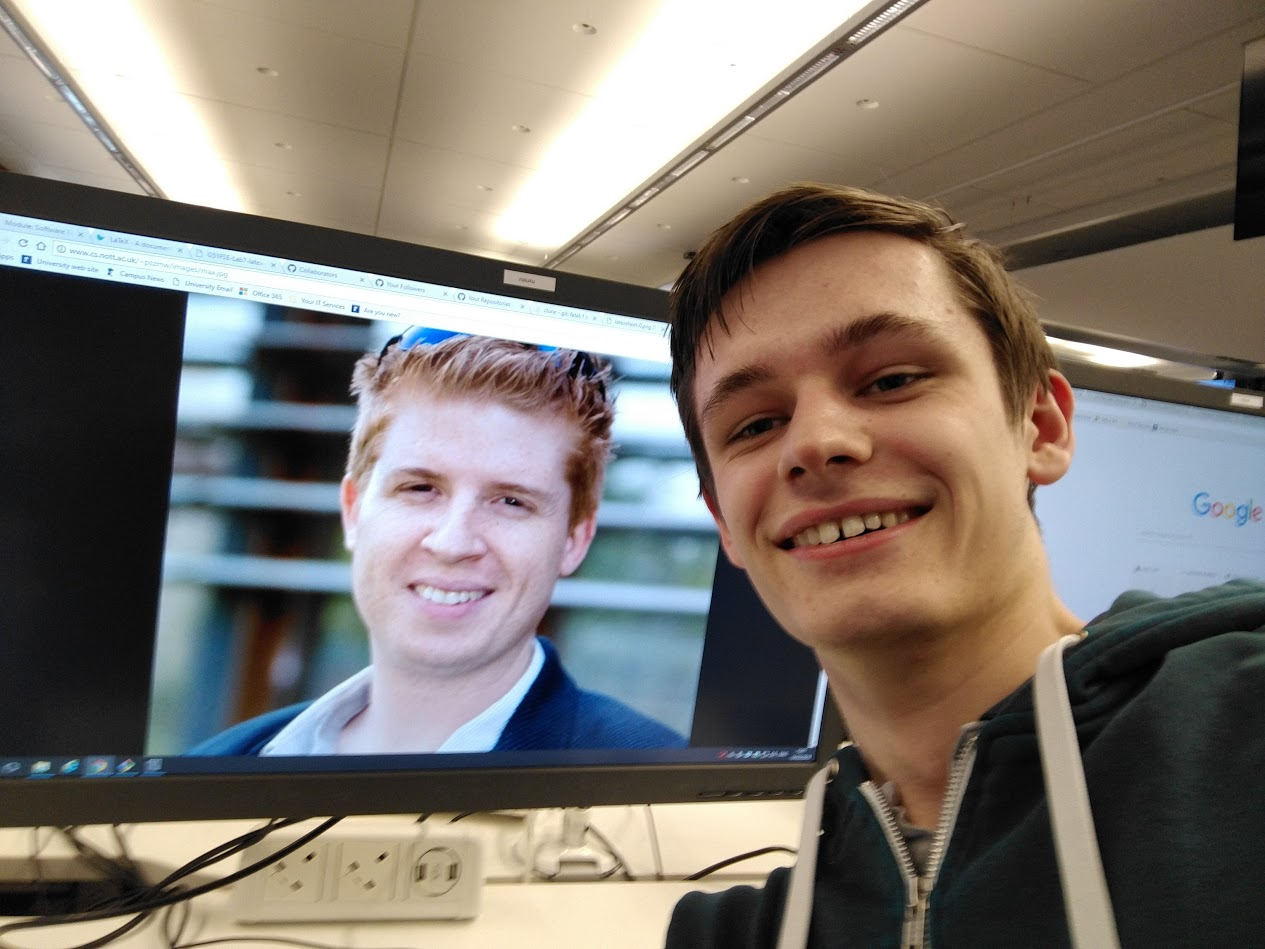
\includegraphics[width=0.5\textwidth]{psytb5_selfie}
\label{fig:selfie}
\end{figure}

You can then use the label of the figure to reference it later with the command ${\backslash}ref$. you can comment out the next line to see an example of how it works.

My selfie with Max is in  Figure~\ref{fig:selfie}.

\subsection{What I have learned in this module}
This is some random text.


\newpage
\include{sections/FifthPart}



\end{document}